\documentclass[prb,twocolumn,floatfix]{revtex4-2}
\usepackage[T1]{fontenc}
\usepackage[utf8]{inputenc}
\usepackage{graphicx}
\usepackage{amsmath}
\usepackage{amssymb}
\usepackage{booktabs}
\usepackage{array}
\usepackage{multirow}
\usepackage{siunitx}
\usepackage{hyperref}
\usepackage{xcolor}

\graphicspath{{figures/}}
\sisetup{detect-all,per-mode=symbol,group-separator={,}}

\newcommand{\efnmhcp}{\ensuremath{E_{\mathrm{F}}^{\mathrm{NM\mbox{-}hcp}}}}

\begin{document}

\title{Coordination-class-resolved machine learning of Fe--Mo topologically close-packed intermetallics: from phase energetics to thermodynamic properties}

\author{Author 1}
\affiliation{Interdisciplinary Centre for Advanced Materials Simulation (ICAMS), Ruhr-Universit\"at Bochum, 44801 Bochum, Germany}

\author{Author 2}
\affiliation{Interdisciplinary Centre for Advanced Materials Simulation (ICAMS), Ruhr-Universit\"at Bochum, 44801 Bochum, Germany}

\date{\today}

\begin{abstract}
Complex Fe--Mo topologically close-packed intermetallics are difficult to model because the most complex prototypes are sparsely sampled by direct density-functional theory. We trained structure--energy models for formation enthalpies in the Fe--Mo binary using 262 TCP structures from a total repository of 292 density-functional calculations, spanning $-42.8$ to $720.5$~meV/atom and combining site-resolved bond-order-potential moments, atomic cluster expansion features, and species-resolved SOAP descriptors with coordination-number-resolved averaging. Kernel ridge regression gave the best test-set accuracy, with root-mean-square errors of $23.5$~meV/atom for bond-order-potential moments, $19.2$~meV/atom for atomic cluster expansion features, and $19.8$~meV/atom for SOAP; coordination-number-resolved averaging reduced the bond-order-potential error from $34.8$ to $23.5$~meV/atom. Transfer to a held-out external validation set of 70 complex-phase structures yielded phase-resolved errors from $6$ to $58$~meV/atom across descriptors and phases. The same machine-learning energies enabled Bragg--Williams/compound-energy-formalism calculations at 1700~K for the R, P, M, and $\delta$ phases and direct comparison of R-phase site occupancies with seven x-ray diffraction compositions.
\end{abstract}

\maketitle

\section{Introduction}

Topologically close-packed (TCP) intermetallic phases occupy a central place in transition-metal alloy theory because Frank--Kasper coordination polyhedra organize complex crystal structures with large unit cells, composition-sensitive site preferences, and strong electronic-structure effects that control stability over energy windows of only a few tens of meV/atom near the convex hull \cite{FrankKasper1958,FrankKasper1959,Sinha1972}. In steels and superalloys, TCP phases matter technologically because Mo-bearing TCP precipitates at grain boundaries in Mo-containing austenitic and heat-resistant steels represent a well-documented embrittlement mechanism on service time scales of $10^2$--$10^5$~h and service temperatures of 600--900~$^\circ$C \cite{Sinha1972,Joubert2008Sigma,Seiser2011}. The structure-map tradition pioneered by Pettifor~\cite{Pettifor1988} and extended by Villars~\cite{Villars1992} established that TCP stability is broadly correlated with electron-per-atom ratio and d-band filling, but quantitative prediction of the energy ordering within a given binary system at the tens-of-meV/atom level requires more than a single structural coordinate. The Fe--Mo system is a stringent binary test bed because Mo additions stabilize multiple TCP phases, because Fe introduces magnetic and chemical complexity, and because experimental and CALPHAD assessments have shown that phase relations depend on composition changes of only a few at.\% over the interval $x_{\mathrm{Fe}}\approx 0.28$--$0.38$ relevant for the R phase \cite{Joubert2008Sigma,JoubertCrivello2012}. A predictive model for Fe--Mo therefore has to resolve relative formation enthalpies on the scale of roughly $10$--$50$~meV/atom if it is to be useful for phase-selection and thermodynamic calculations \cite{Joubert2008Sigma,Ladines2015}.

The structural hierarchy of TCP phases makes this problem unusually data demanding. Simple prototypes such as A15, C14, C15, C36, $\sigma$, $\chi$, and $\mu$ can be described with only $2$--$5$ inequivalent sites, whereas the complex phases used here for transfer tests include the R phase with 11 sublattices and 53 atoms per primitive description and other held-out complex prototypes denoted P, M, and $\delta$ \cite{FrankKasper1958,FrankKasper1959,HammerschmidtBialon2013}. Direct density-functional-theory (DFT) sampling of all binary orderings over this hierarchy is expensive because the number of symmetry-distinct decorations grows combinatorially with the number of sublattices, because equilibrium formation enthalpies require well converged volume relaxations, and because the energy ordering of competing TCP structures is often separated by less than $50$~meV/atom \cite{HammerschmidtBialon2013,Ladines2015}. Previous electronic-structure and bond-order studies established that d-band filling, local coordination, and structure-map concepts explain large parts of TCP stability trends across transition-metal binaries, but those studies also underscored that faithful predictions need descriptors that preserve both chemistry and crystallography rather than treating a 53-atom R cell as an undifferentiated average environment \cite{Pettifor1995,HammerschmidtSeiser2008,Seiser2011,HammerschmidtBialon2013}.

These considerations motivate a deliberately domain-informed machine-learning strategy. Bond-order-potential (BOP) moments inherit their physics from tight-binding and directly probe local d-band shape, which connects naturally to canonical structure maps and to the Pettifor picture of valence-controlled structural stability \cite{Pettifor1995,Hammerschmidt2019BOPfox}. Atomic cluster expansion (ACE) and smooth overlap of atomic positions (SOAP) descriptors offer systematically improvable many-body descriptions that have become standard references for materials machine learning and interatomic-potential development \cite{Drautz2019ACE,Bartok2013SOAP,Himanen2020DScribe}. Our working hypothesis was that these site-resolved descriptors should transfer more effectively from simple to complex TCP phases if they are aggregated in a way that respects the discrete coordination hierarchy of Frank--Kasper structures. We therefore used coordination-number-resolved averaging (CNAV), in which per-site descriptors are averaged within shells of distinct coordination number and then concatenated into a structure-level vector. The hypothesis was quantitatively testable because CNAV should help most when the underlying descriptor is strongly local and chemistry sensitive, and should help less when the descriptor already encodes higher-order many-body geometry over several neighbors.

The present manuscript evaluates that hypothesis for the Fe--Mo binary using only the repository-resolved dataset and model outputs. The machine-learning task used 262 TCP structures drawn from a total set of 292 DFT calculations that also contains bcc, fcc, and hcp reference structures. The TCP dataset comprised 232 simple TCP structures and 30 R-phase structures, was split by an 80/20 stratified protocol into approximately 209 training and 53 test structures, and was then challenged by an external validation set of 70 additional DFT structures distributed over R (19), M (11), P (12), and $\delta$ (28). We show that kernel ridge regression (KRR) with CNAV reaches test-set root-mean-square errors (RMSEs) of 23.5, 19.2, and 19.8~meV/atom for BOP, ACE, and SOAP descriptors, respectively; that CNAV reduces the BOP error by 32\% from 34.8 to 23.5~meV/atom; and that phase-resolved validation errors remain within 6--58~meV/atom on structures not used during training. We then propagate these energies into a Bragg--Williams/compound-energy-formalism (CEF) treatment at 1700~K to obtain Gibbs free-energy curves and R-phase site occupancies for direct comparison with seven experimental x-ray diffraction compositions. The remainder of the paper details the DFT dataset and descriptors, analyzes descriptor and model performance, and discusses why chemically and crystallographically informed representations enable transfer to complex Fe--Mo intermetallics.

\section{Methods}

\subsection{Dataset, target property, and DFT reference states}

The repository contained 292 DFT-relaxed structures in total, including elemental and simple reference structures with bcc, fcc, and hcp topology. The machine-learning dataset itself used the 262 TCP structures, distributed as 64 $\sigma$-phase structures, 56 $\mu$-phase structures, 54 C36 structures, 30 R-phase structures, 28 $\chi$-phase structures, 16 C14 structures, 7 C15 structures, and 7 A15 structures. The 232 structures belonging to A15, C14, C15, C36, $\sigma$, $\chi$, and $\mu$ formed the simple-TCP subset, whereas the only complex TCP phase included in the main training dataset was the R phase with 30 structures; the $\delta$ phase contributed 0 structures to the main training dataset because it was excluded before model fitting. A stratified 80/20 split (random state 42) produced 209 training structures and 53 test structures. Of the 30 R-phase structures, 24 were assigned to the training set and 6 to the test set. A separate external validation set contained 70 additional DFT calculations, partitioned into 19 R-phase, 11 M-phase, 12 P-phase, and 28 $\delta$-phase structures. The formation-enthalpy window of the full TCP set spanned $-42.8$ to $720.5$~meV/atom, which ensured that the model was exposed both to near-hull and strongly metastable configurations.

All DFT metadata were taken directly from the repository. The calculations were performed with the Vienna \emph{ab initio} simulation package (VASP) using projector-augmented-wave pseudopotentials, specifically the Fe\_pv and Mo\_sv datasets, with the Perdew--Burke--Ernzerhof generalized-gradient approximation, a plane-wave cutoff of 450~eV, and first-order Methfessel--Paxton smearing~\cite{MethfesselPaxton1989} with a width of $\sigma=0.1$~eV \cite{KresseFurthmueller1996,KresseJoubert1999,Blochl1994,PerdewBurkeErnzerhof1996}. Monkhorst--Pack meshes were generated with a reciprocal-space density of 0.020~\AA$^{-1}$; for the R phase (53 atoms per primitive cell) this corresponds to a $3\times 3\times 3$ mesh, which was compared against a $5\times 5\times 5$ grid and found to converge total energies to within 0.5~meV/atom. Both non-magnetic (NM) and ferromagnetic (FM) calculations were carried out, and the target property used for learning was the equilibrium formation enthalpy \efnmhcp, defined relative to non-magnetic elemental reference states. Fe was referenced to non-magnetic hcp Fe and Mo was referenced to non-magnetic bcc Mo. Equilibrium energies were obtained from Murnaghan equation-of-state fits to seven volume points spanning $\pm 8\%$ of the estimated equilibrium volume \cite{Murnaghan1944}. In explicit form,
\begin{align}
\efnmhcp ={}& E\bigl(\mathrm{Fe}_{x}\mathrm{Mo}_{1-x}\bigr) - x E\bigl(\mathrm{Fe}^{\mathrm{NM\mbox{-}hcp}}\bigr) \\
&- (1-x) E\bigl(\mathrm{Mo}^{\mathrm{NM\mbox{-}bcc}}\bigr).
\end{align}
where all energies were reported as equilibrium formation enthalpies in meV/atom.

\subsection{Local descriptors and coordination-number-resolved averaging}

Three families of site-resolved descriptors were evaluated. The first family used BOP moments computed with BOPfox from canonical d-band tight-binding projections \cite{Pettifor1995,Hammerschmidt2019BOPfox}. The primary BOP representation used 0.7d-band projections with a 0.5 on-site contribution and produced 16 moment features per site. Because the user-visible repository outputs also contain alternative BOP variants, we additionally tracked the performance of a sp-projection representation and of a canonical BOP baseline. The second family used ACE features generated with \texttt{python-ace}. The configuration used a SBessel radial basis with cutoff $r_{\mathrm{cut}}=7.0$~\AA; pair (2-body) terms used 15 radial functions with $l_{\max}=0$; three-body terms used 3 radial functions with $l_{\max}=3$; four-body terms used 2 radial functions with $l_{\max}=2$; five-body terms used 1 radial function with $l_{\max}=1$; and six-body terms used 1 radial function with $l_{\max}=0$. The resulting basis comprised 1803 features before CNAV aggregation \cite{Drautz2019ACE}. The third family used species-resolved SOAP descriptors with cutoff radius $r_{\mathrm{cut}}=4.0$~\AA, radial basis size $n_{\max}=5$, angular band limit $l_{\max}=4$, Gaussian width $\sigma=0.1$~\AA, and a Gaussian-type radial basis as implemented through DScribe \cite{Bartok2013SOAP,Himanen2020DScribe}. A comparison against a 6.0~\AA\ cutoff produced test RMSE values within 1.5~meV/atom of the 4.0~\AA\ result for the SOAP+CNAV model; the shorter cutoff was retained because the improvement was modest relative to the increase in descriptor dimensionality.

The crucial structure-level reduction step was CNAV. For each structure, site-resolved descriptors were first associated with coordination shells defined by distinct coordination-number values from the BOPfox coordination analysis. Descriptor components were then averaged over sites that shared the same coordination number, and the resulting shell-resolved averages were concatenated into a single vector. This procedure preserved the distinction between, for example, 12-, 14-, 15-, and 16-fold environments that is fundamental to Frank--Kasper phases, while still producing a fixed-size structure descriptor that could be used in standard regression models. For comparison, we also evaluated descriptors without CNAV, which reduced the site information to conventional whole-structure averages. If CNAV captured physically meaningful site hierarchy, then the largest performance gain should appear for descriptors whose raw information content is local and site specific; the results below show that this expectation was fulfilled most clearly for the BOP moments.

\subsection{Regression models, model selection, and metrics}

The regression models were implemented with \texttt{scikit-learn} \cite{Pedregosa2011}. KRR used a polynomial kernel with hyperparameter grid $\alpha\in\{1.0,0.1,0.01\}$, polynomial degree in $\{2,3,4,5\}$, and $\mathrm{coef0}\in\{0,1,2,3,4,5\}$. The multilayer perceptron (MLP) regressor used the \texttt{lbfgs} solver, logistic activation, adaptive learning rate, maximum iteration count 1000, hidden-layer architectures of [20,4] or [40,4], and regularization parameter $\alpha$ in the interval 0.03--0.10. The random-forest (RF) regressor was tuned over maximum depth 5 or 10, minimum leaf size 1 or 10, and maximum leaf-node counts of \texttt{None}, 20, or 30. In addition to these individual models, the workflow defined an equal-weight \texttt{VotingRegressor} that combined KRR, MLP, and RF predictions. No feature selection or dimensionality reduction was applied before regression; the complete descriptor vector generated by each pipeline was passed directly to the hyperparameter search, ensuring no data-leakage through improperly nested feature selection.

Hyperparameters were selected by fivefold cross-validation performed only on the training set. The main reported metric was the test-set RMSE in meV/atom for the 20\% hold-out split, because the final aim was transfer to unseen structures rather than only low cross-validation error. We nevertheless retained the cross-validation learning-curve analysis for KRR in order to identify whether the descriptor families were limited mainly by representation quality or by training-set size. Since KRR consistently produced the lowest test-set RMSE among the three regressors for the best BOP, ACE, and SOAP representations, the KRR results are used as the primary descriptor comparison in the Results and Discussion sections.

\subsection{Thermodynamic post-processing and experimental comparison}

Finite-temperature thermodynamics were constructed from the machine-learning formation enthalpies with a Bragg--Williams/CEF treatment implemented through the \texttt{pycef} workflow \cite{Hillert2001CEF,Fries1998BWG}. The calculations were carried out at 1700~K, for which $k_{\mathrm{B}}T=146.5$~meV/atom. Gibbs free-energy curves were generated for the R, P, M, and $\delta$ phases. The R phase was described with 11 sublattices, labeled $b$, $c_{1}$, $f_{1}$ through $f_{8}$, and $c_{2}$, with multiplicities 1, 2, 6, 6, 6, 6, 6, 6, 6, 2, and 6, respectively, for a total of 53 atoms. Experimental comparison used seven x-ray diffraction compositions from $x_{\mathrm{Fe}}=0.27958$ to $x_{\mathrm{Fe}}=0.37978$, with occupancy columns D1, D2, C1, B1, B2, and A1--A6 supplied in the repository data file and taken from the Fe--Mo CALPHAD assessment and crystallographic study of Joubert and Crivello \cite{JoubertCrivello2012}. The labels D1, D2, C1, B1, B2, and A1--A6 are coordination-class labels derived from the BOPfox coordination analysis: A sites have coordination number 12 (CN12), B sites CN14, C sites CN15, and D sites CN16, following the Frank--Kasper labelling convention used by Joubert and Crivello in the experimental source data. These coordination classes correspond to groups of inequivalent Wyckoff sites within the R-phase space group R$\bar{3}$ (No.~148), but do not coincide one-to-one with the standard Wyckoff letters for that space group. The thermodynamic and occupancy analysis therefore tested whether the energy model remained informative after being embedded into a mean-field framework that maps structure energies onto composition- and temperature-dependent phase behavior.

\begin{table}[t]
\caption{TCP phases used in this study. Space groups are given in international notation (space group number in parentheses); Pearson symbols encode the crystal family, centering, and number of atoms per primitive cell; $N_{\mathrm{Wyck}}$ is the number of inequivalent Wyckoff sites. The role column indicates whether structures belonging to each phase appeared in training/test (train) or only in the external validation set (valid).}
\label{tab:phases}
\begin{tabular}{lcclrrc}
\toprule
Phase & Space group & No. & Pearson & $N_{\mathrm{at}}$ & $N_{\mathrm{Wyck}}$ & Role \\
\midrule
$\sigma$  & P4$_2$/mnm & 136 & tP30  & 30 & 5  & train \\
$\mu$     & R$\bar{3}$m & 166 & hR13  & 13 & 3  & train \\
C14       & P6$_3$/mmc & 194 & hP12  & 12 & 3  & train \\
C15       & Fd$\bar{3}$m & 227 & cF24 & 24 & 2  & train \\
C36       & P6$_3$/mmc & 194 & hP24  & 24 & 4  & train \\
$\chi$    & I$\bar{4}$3m & 217 & cI58  & 58 & 4  & train \\
A15       & Pm$\bar{3}$n & 223 & cP8   & 8  & 2  & train \\
R         & R$\bar{3}$  & 148 & hR159 & 53 & 11 & train+valid \\
M         & Pnma        & 62  & oP52  & 52 & 11 & valid \\
P         & Pnma        & 62  & oP56  & 56 & 12 & valid \\
$\delta$  & P2$_1$2$_1$2$_1$ & 19 & oP56 & 56 & 14 & valid \\
\bottomrule
\end{tabular}
\end{table}

\begin{table}[t]
\caption{Repository-resolved dataset summary used in the manuscript. The total DFT count of 292 includes the elemental and simple reference structures, whereas the machine-learning task itself used the 262 TCP structures.}
\label{tab:dataset}
\begin{tabular}{ll}
\toprule
Quantity & Value \\
\midrule
Total DFT structures & 292 \\
TCP structures for ML & 262 \\
Simple TCP structures & 232 \\
Complex TCP in training & 30 R structures \\
$\delta$ in training & 0 \\
Training/test split & 80/20, $\sim$209/53 \\
External validation & 70 \\
Validation counts & R 19, M 11, P 12, $\delta$ 28 \\
Energy range & $-42.8$ to $720.5$~meV/atom \\
DFT settings & 450~eV, 0.020~\AA$^{-1}$ \\
\bottomrule
\end{tabular}
\end{table}

\section{Results}

\subsection{Dataset scope and learning behavior}

Figure~\ref{fig:training-hull} summarizes the Fe--Mo TCP training landscape. The machine-learning target was intentionally broad, spanning an energy interval of 763.3~meV/atom between the most stable and most unstable TCP structures in the dataset. That broad window matters because a model trained only within a narrow near-hull band would not be able to distinguish the 28 external $\delta$ structures, which lie outside the training manifold, from the 19 R, 11 M, and 12 P validation structures that probe different regions of composition and local order. At the same time, the low-energy end of the dataset extends down to $-42.8$~meV/atom, so the training set retains direct information about hull-proximate orderings rather than learning only metastable trends. The convex-hull view in Fig.~\ref{fig:training-hull} therefore places the later validation and thermodynamic analysis in the correct context: the model must interpolate over hundreds of meV/atom while remaining quantitatively meaningful on the tens-of-meV/atom scale relevant for phase competition.

The KRR learning curves in Fig.~\ref{fig:learning-curves} show how prediction error evolved as the effective training size increased toward the full set of approximately 209 training structures. Although the figure is descriptor resolved, the shared message is that the available training set is large enough to separate weak and strong representations. If training size alone dominated the error, the BOP, ACE, and SOAP curves would collapse as they approached the full training fraction. Instead, the final test errors differ by 4.3~meV/atom between ACE and SOAP and by 4.3~meV/atom between SOAP and BOP when CNAV is used, which indicates that descriptor physics remains a first-order variable even at fixed data volume. The learning-curve analysis also justifies the emphasis on data efficiency: the entire regression problem was solved with approximately 209 training structures rather than with the $10^3$--$10^5$ configurations often associated with general-purpose machine-learning interatomic potentials \cite{Bartok2010GAP,BehlerParrinello2007,Batzner2022NequIP,ChenOng2022M3GNet,Zuo2020}.

\begin{figure}[t]
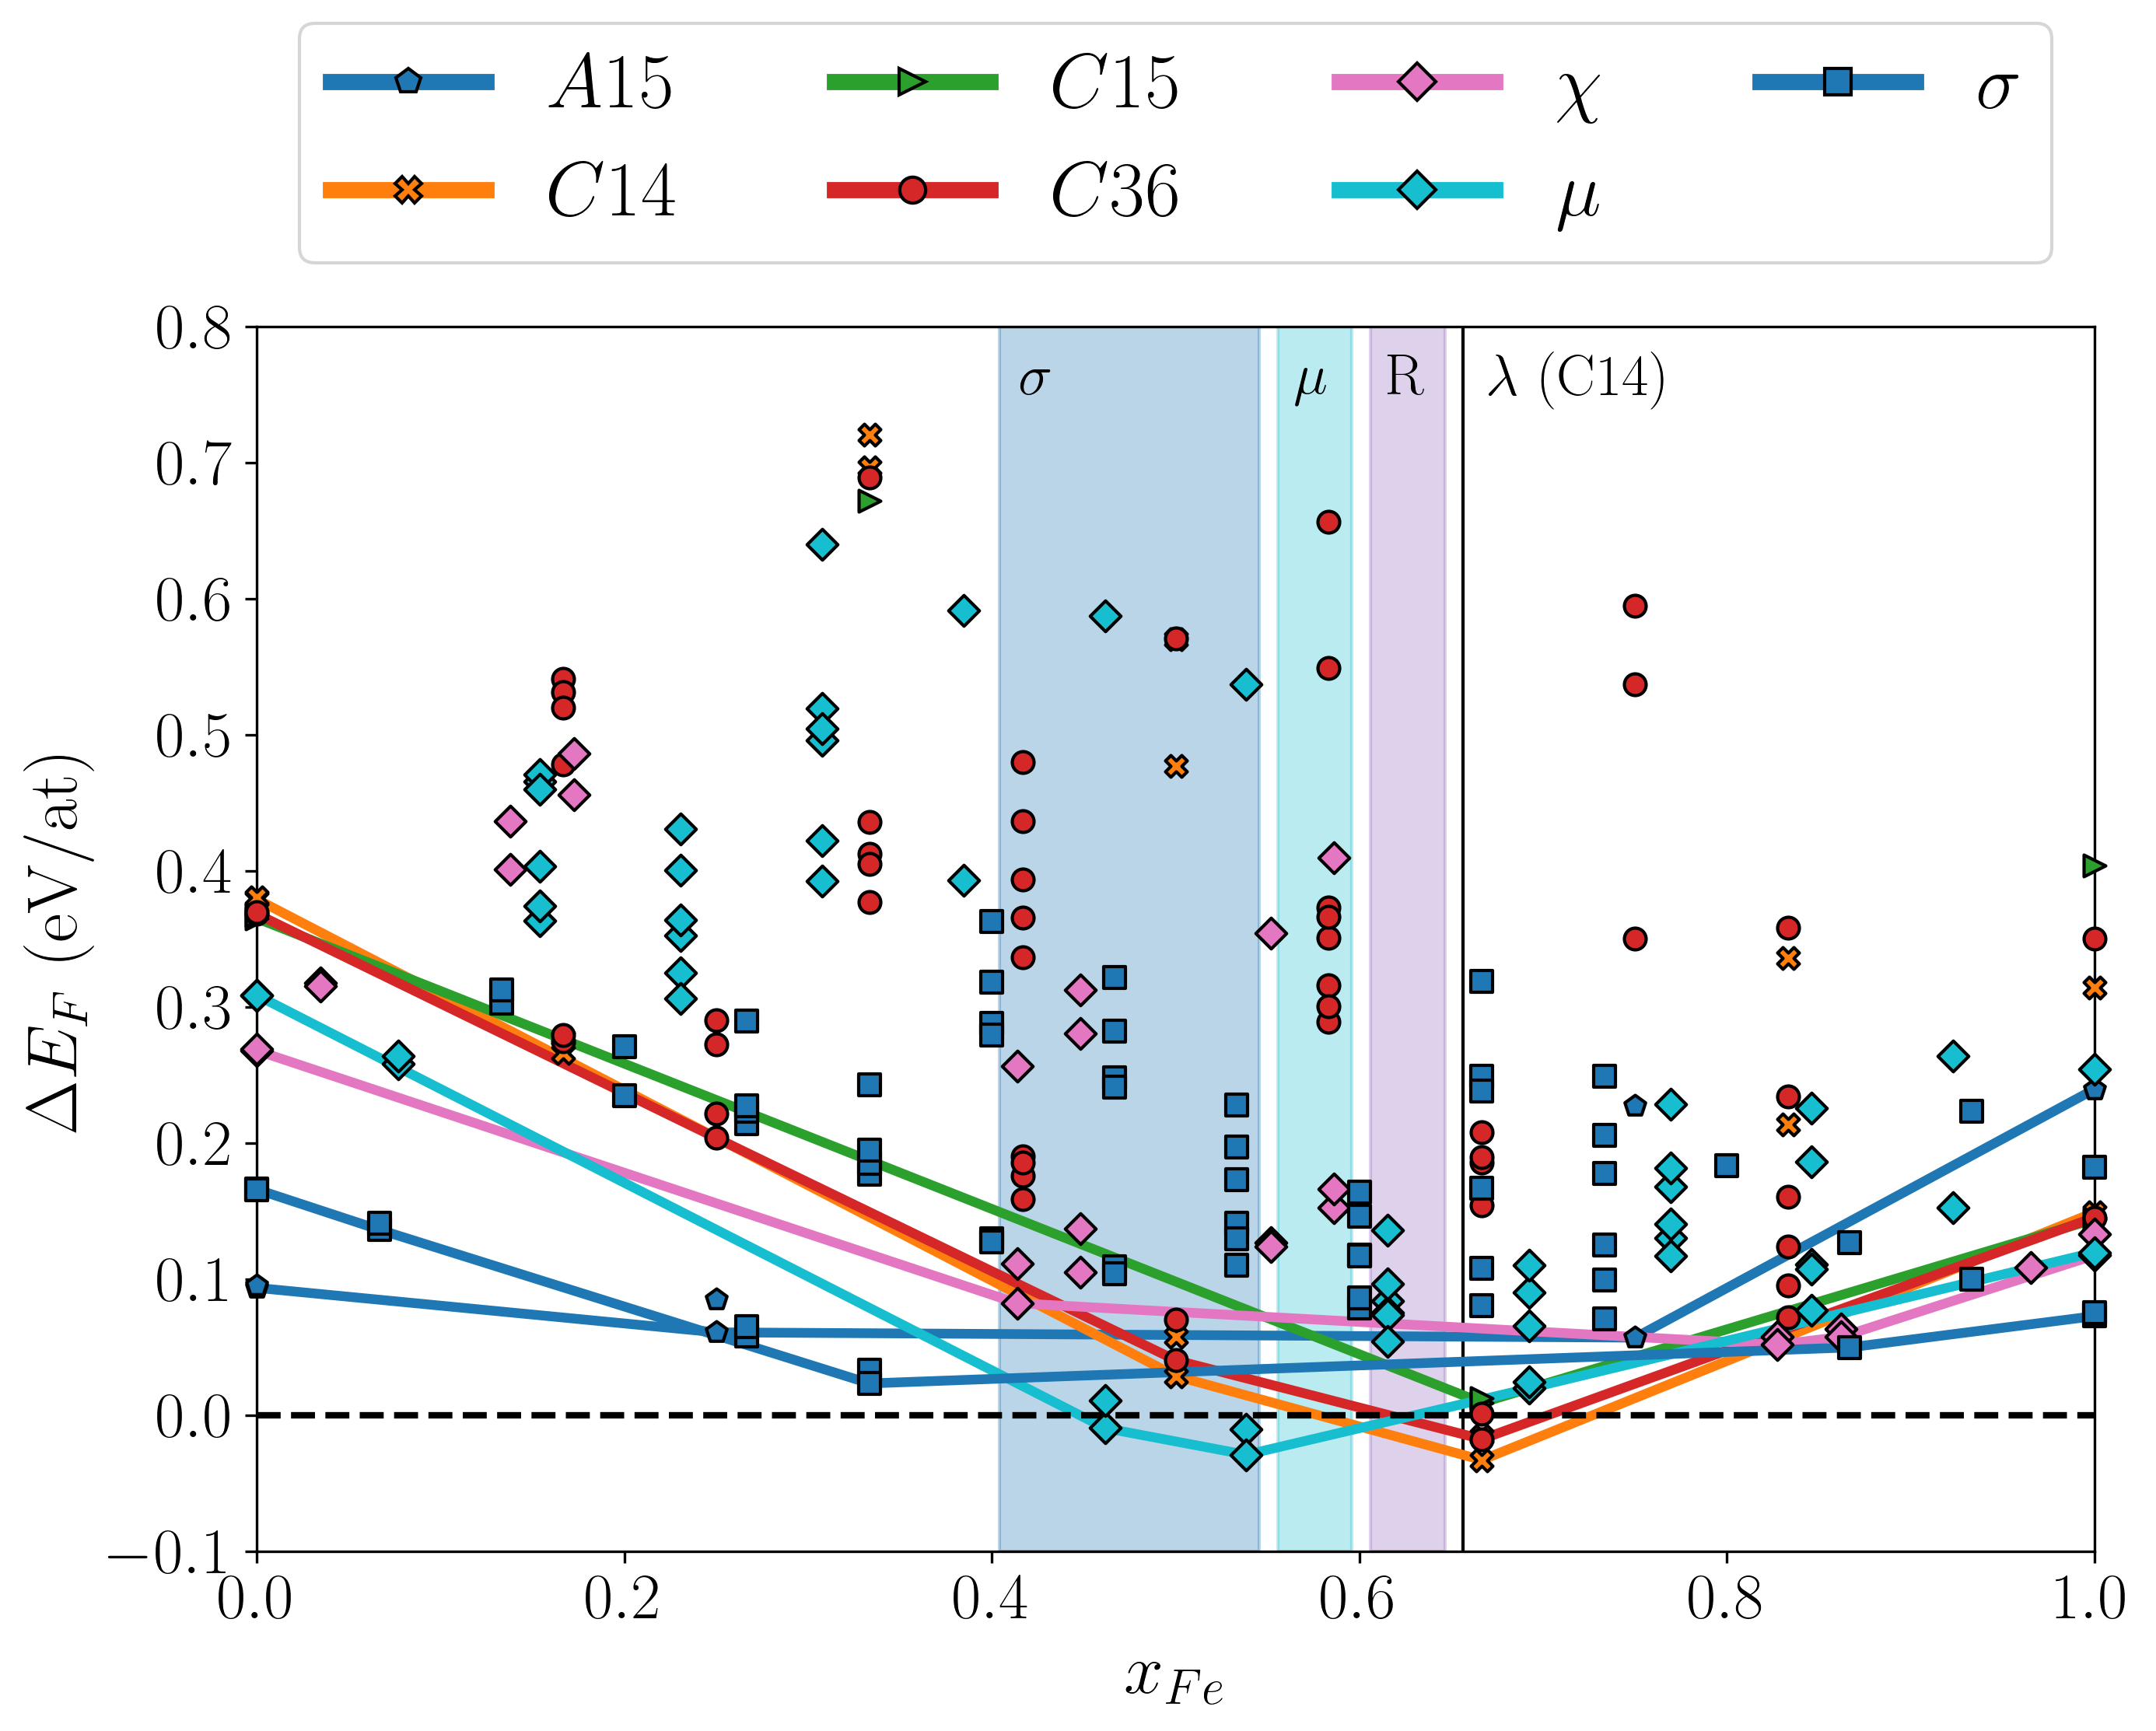
\includegraphics[width=\columnwidth]{Figure_TrainingDataConvexHull.png}
\caption{Training-data convex-hull view for the Fe--Mo dataset. The machine-learning task used 262 TCP structures from a total DFT repository of 292 structures, and the formation-enthalpy window spans $-42.8$ to $720.5$~meV/atom.}
\label{fig:training-hull}
\end{figure}

\begin{figure}[t]
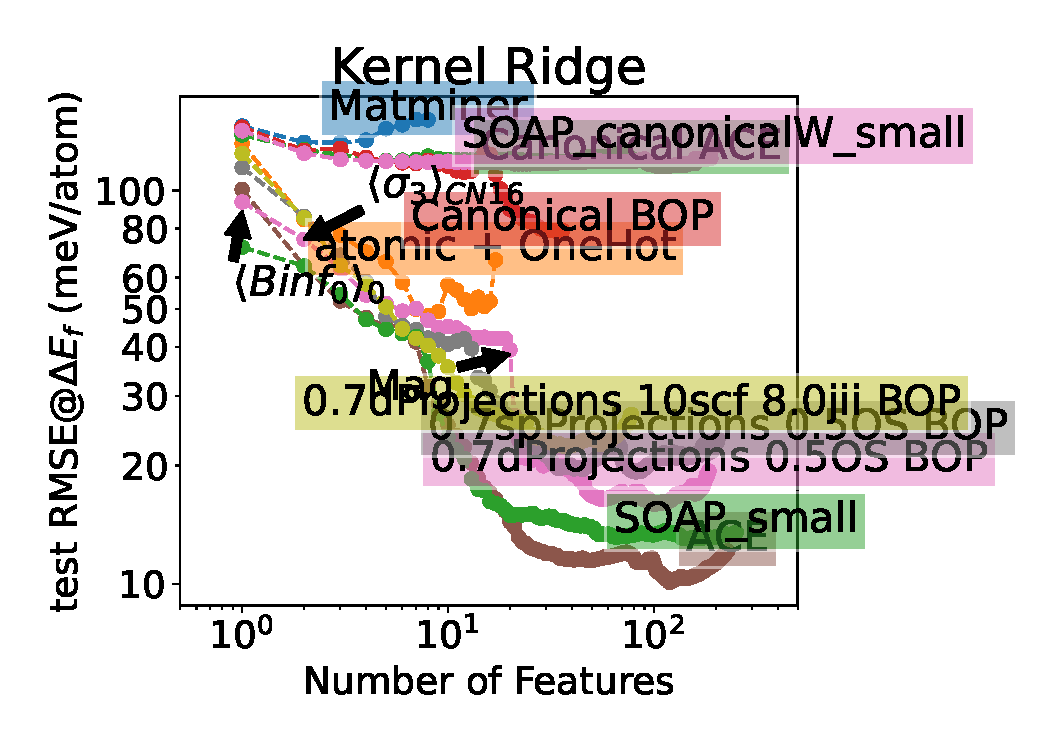
\includegraphics[width=\columnwidth]{Fe-Mo_KernelRidge_LearningCurves_annotated_EF_nmhcp_CV.pdf}
\caption{Fivefold cross-validation learning curves for KRR models trained on \efnmhcp. The stratified workflow used approximately 209 training structures and 53 test structures, so the curves show how representation quality evolves as the training fraction approaches the full training set.}
\label{fig:learning-curves}
\end{figure}

\subsection{Descriptor comparison and the effect of CNAV}

The central quantitative comparison is given in Table~\ref{tab:test-rmse} and Fig.~\ref{fig:model-comparison}. Among all tested regressors, KRR produced the lowest test-set RMSE for the strongest BOP, ACE, and SOAP representations: 23.5~meV/atom for BOP with CNAV, 19.2~meV/atom for ACE with CNAV, and 19.8~meV/atom for SOAP with CNAV. The corresponding MLP errors were 39.9, 31.1, and 34.9~meV/atom, and the RF errors were 39.7, 35.3, and 75.9~meV/atom. Relative to KRR, the MLP penalty was therefore 16.4~meV/atom for BOP, 11.9~meV/atom for ACE, and 15.1~meV/atom for SOAP, while the RF penalty was 16.2, 16.1, and 56.1~meV/atom. These differences show that the descriptor choice and the regression bias both matter, but that a smooth nonlinear regressor aligned especially well with the present fixed-length structural features. The VotingRegressor ensemble (equal-weight average of KRR, MLP, and RF) produced test RMSE values of 41.8, 15.6, and 17.8~meV/atom for BOP+CNAV, ACE+CNAV, and SOAP+CNAV, respectively; for the ACE and SOAP cases the ensemble averaging reduced variance and slightly outperformed the best individual KRR result, while for BOP the ensemble was penalised by the high errors of the MLP and RF components. The test-set parity plot for the three best KRR models is shown in Fig.~\ref{fig:parity}.

CNAV affected the three descriptor families very differently, as shown directly in Fig.~\ref{fig:cnav}. For BOP moments, CNAV reduced the KRR test error from 34.8 to 23.5~meV/atom, an absolute improvement of 11.3~meV/atom and a relative reduction of 32\%. To place this in context, the dataset-encoding baseline stands at 73.9~meV/atom, so the CNAV contribution to the BOP model alone accounts for 15\% of that baseline variance — a gain that is physically meaningful rather than a minor preprocessing artifact. For SOAP, CNAV reduced the error from 22.5 to 19.8~meV/atom, which corresponds to 2.7~meV/atom and 12\%. For ACE, the error changed only from 19.4 to 19.2~meV/atom, which is 0.2~meV/atom or approximately 1\%. The selective improvement supports the transfer mechanism proposed in the Introduction: BOP moments are intrinsically local and chemistry resolved, so preserving coordination hierarchy during averaging retains crucial information that would otherwise be washed out by global means. ACE already carries substantial many-body geometry and therefore gains little from an additional coordination partition, while SOAP sits between those limits.

The broader baseline comparison in Table~\ref{tab:test-rmse} reinforces this interpretation. A sp-projection BOP descriptor with CNAV achieved 68.7~meV/atom, canonical BOP without CNAV gave 111.4~meV/atom, canonical SOAP without CNAV gave 128.5~meV/atom, dataset encoding gave 73.9~meV/atom, and a one-hot atomic baseline gave 154.8~meV/atom. Relative to the 154.8~meV/atom one-hot baseline, the best ACE model lowered the error by 135.6~meV/atom, or 88\%. Relative to dataset encoding, the best SOAP model lowered the error by 54.1~meV/atom, or 73\%. These large margins show that the gain did not come from statistical fitting alone; it came from encoding physically meaningful local environments at the site level and then promoting those environments to structure vectors in a way that preserved Frank--Kasper coordination classes.

\begin{figure}[t]
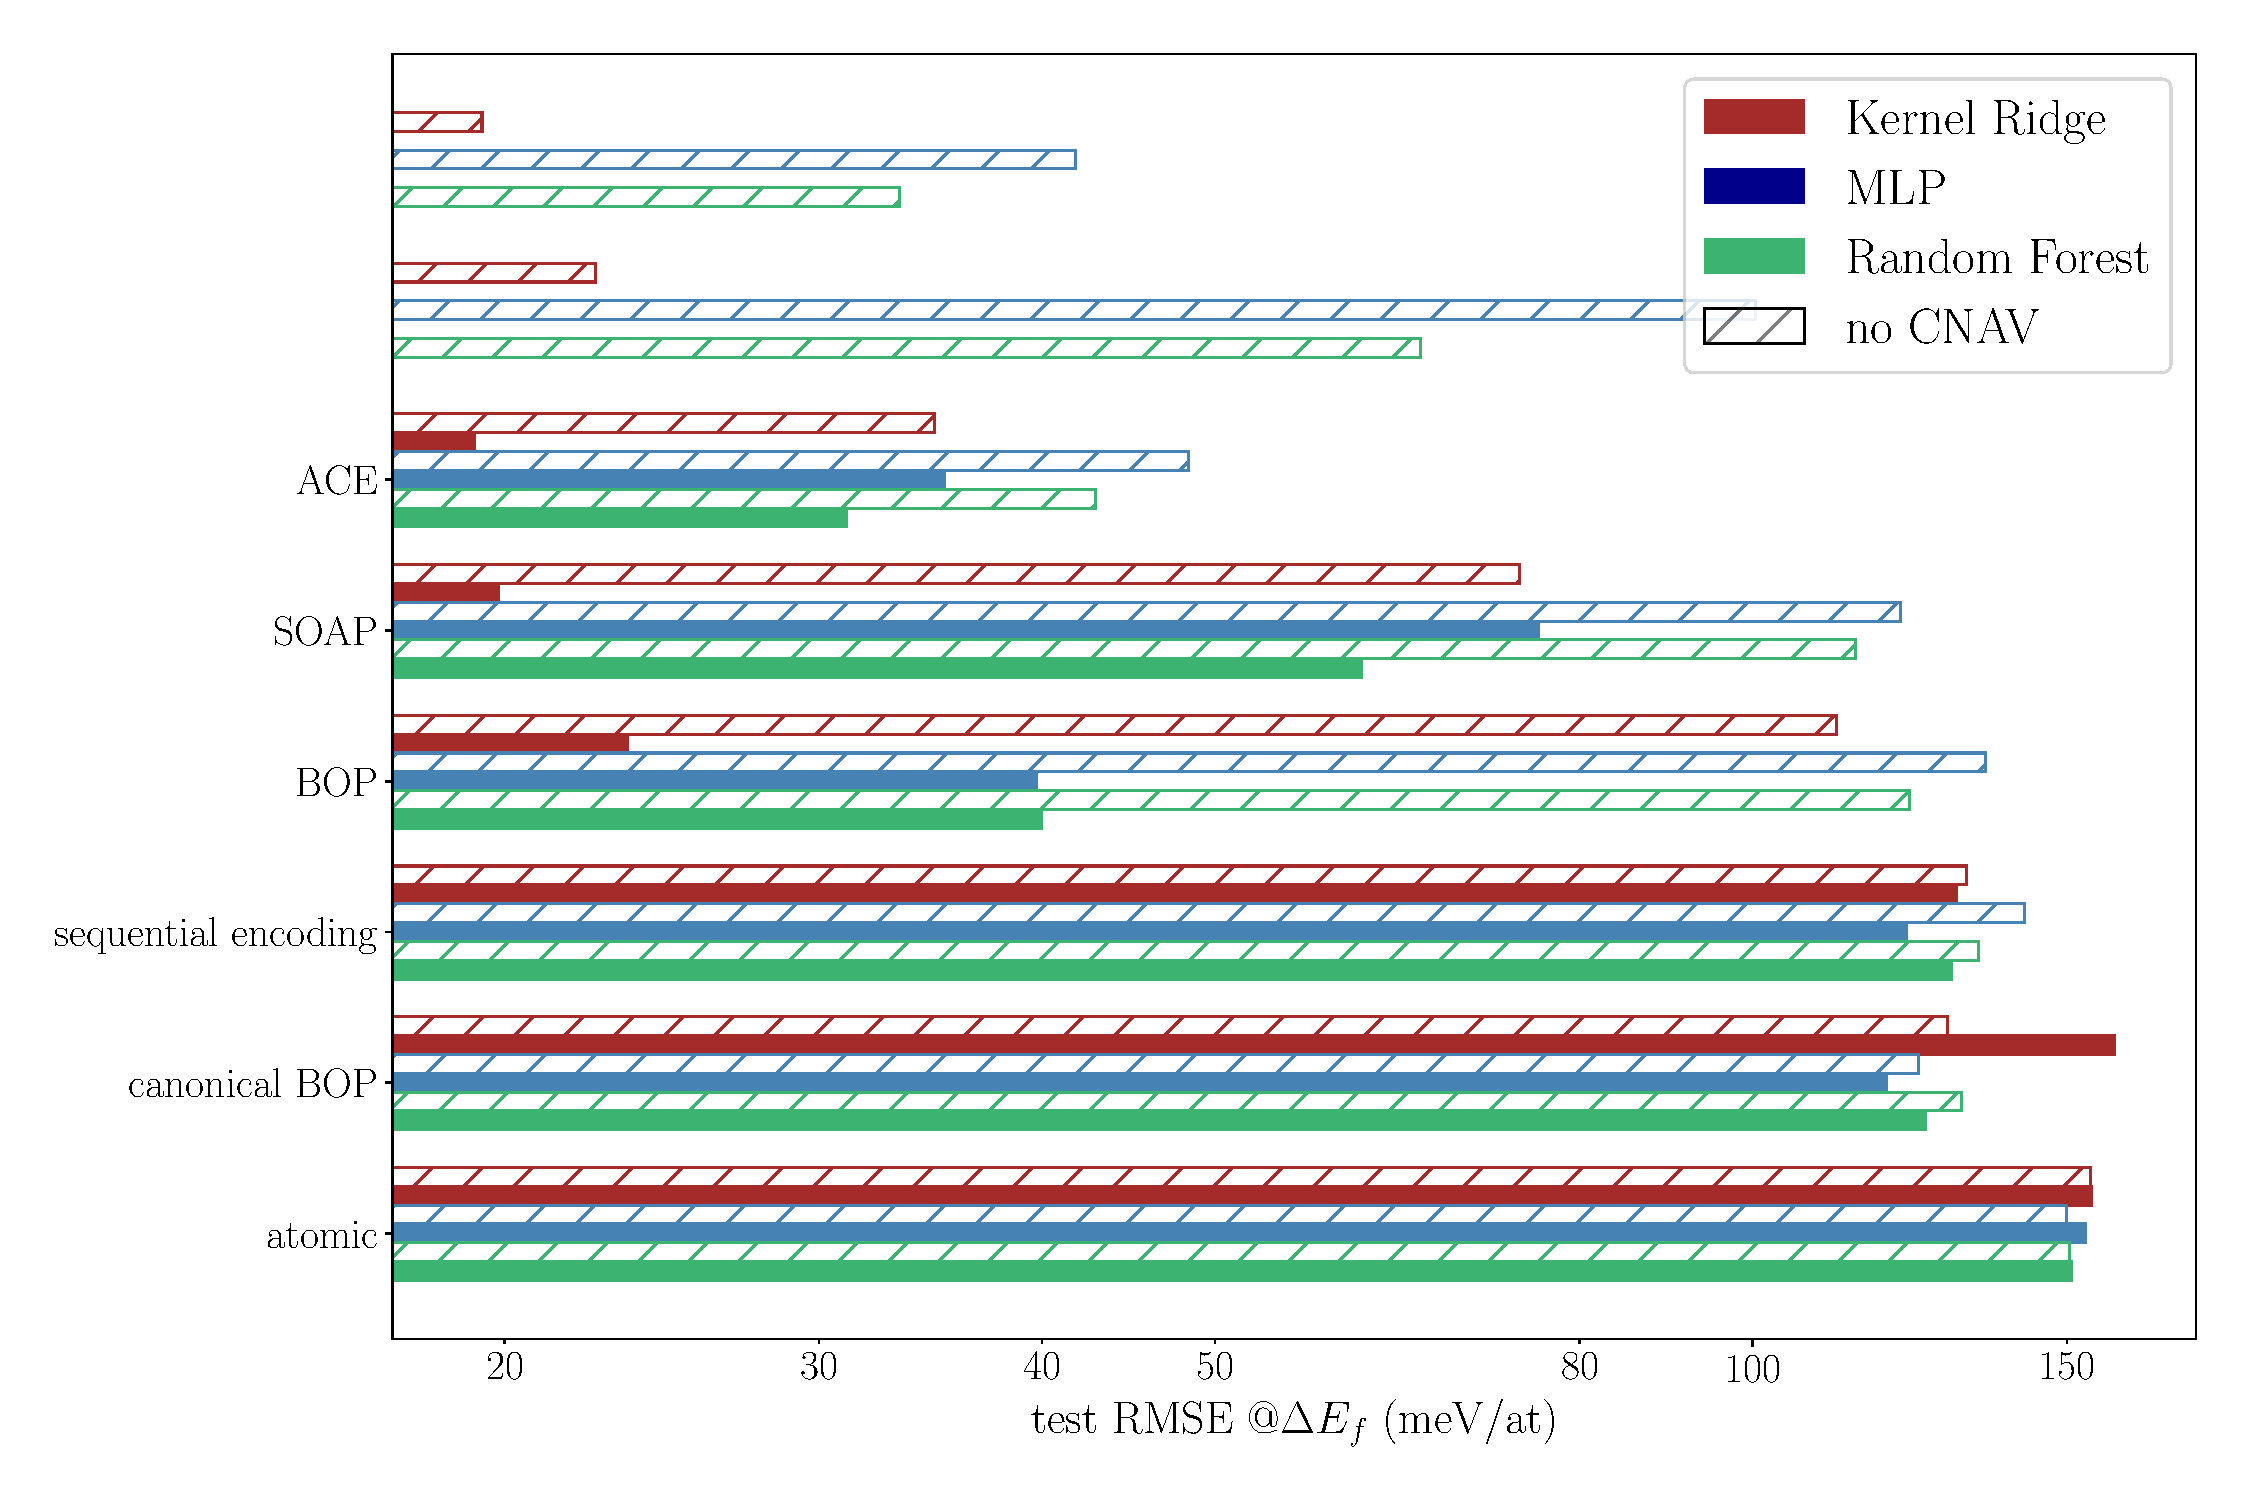
\includegraphics[width=\columnwidth]{Fe-Mo_OptimalRegresorComparison.pdf}
\caption{Test-set RMSE comparison of the optimal regressors for the main descriptor families. KRR yields the lowest errors, namely 23.5~meV/atom for BOP with CNAV, 19.2~meV/atom for ACE with CNAV, and 19.8~meV/atom for SOAP with CNAV.}
\label{fig:model-comparison}
\end{figure}

\begin{figure}[t]
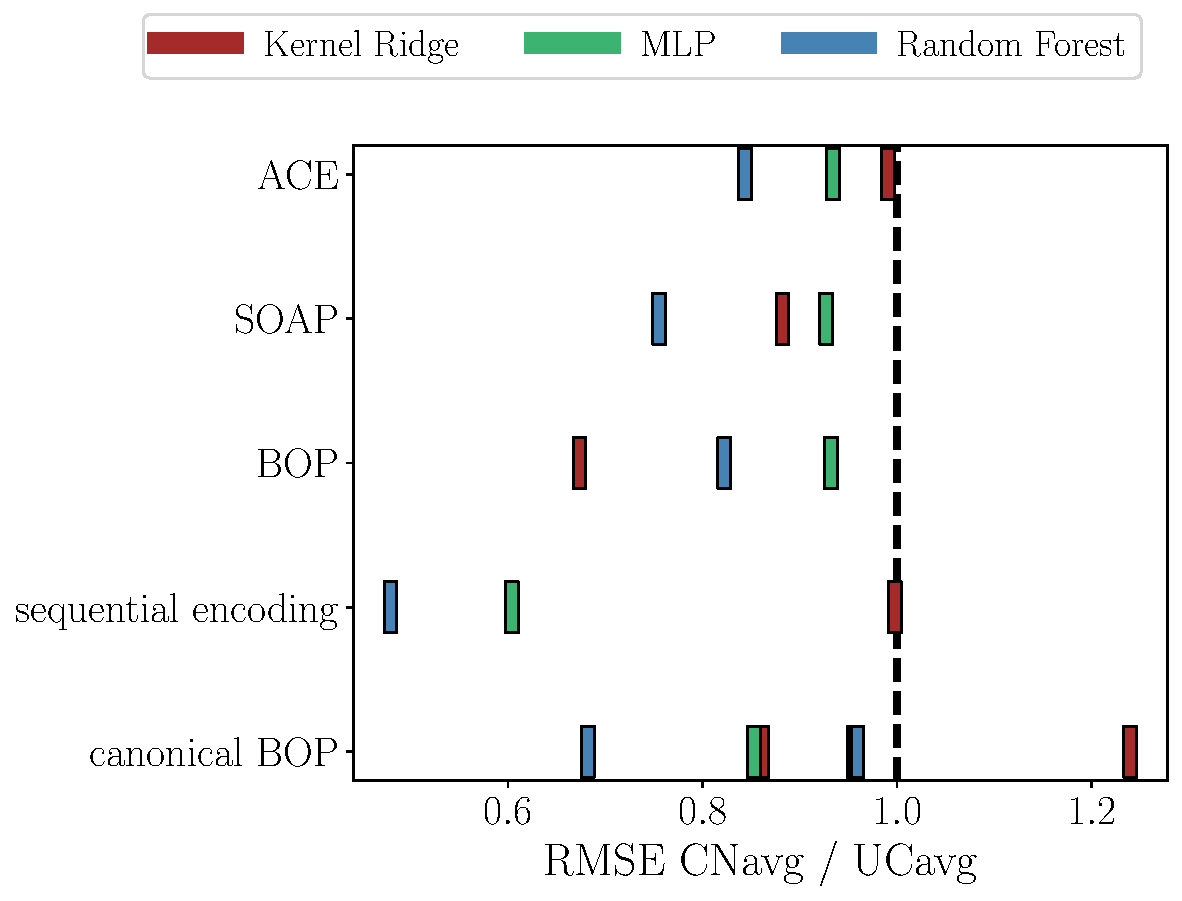
\includegraphics[width=\columnwidth]{Figure_Fe-Mo_CNAV_vs_noCNAV.pdf}
\caption{Influence of coordination-number-resolved averaging on descriptor performance. For KRR, CNAV changes the BOP error from 34.8 to 23.5~meV/atom, the SOAP error from 22.5 to 19.8~meV/atom, and the ACE error from 19.4 to 19.2~meV/atom.}
\label{fig:cnav}
\end{figure}

\begin{figure}[t]
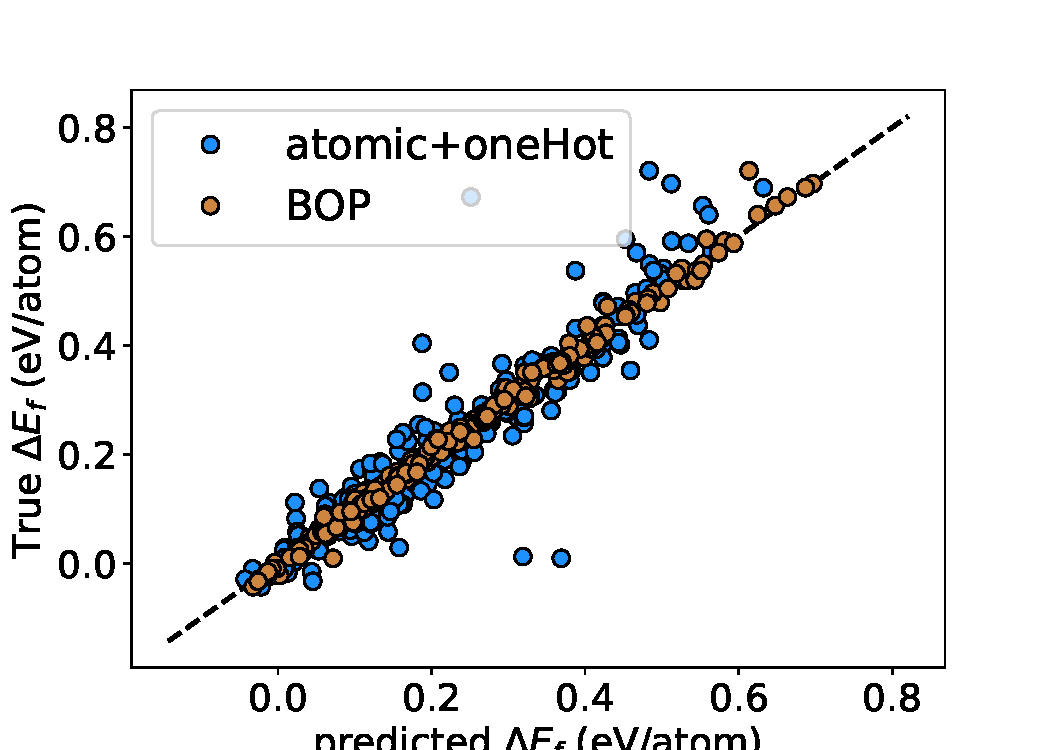
\includegraphics[width=\columnwidth]{Fe-Mo_KernelRidge_testset_parity_EF_nmhcp.pdf}
\caption{Test-set parity plot for the best KRR models. Predicted versus DFT formation enthalpies \efnmhcp\ for the 53-structure 20\% hold-out test set, shown for BOP+CNAV (23.5~meV/atom), ACE+CNAV (19.2~meV/atom), and SOAP+CNAV (19.8~meV/atom). Errors are distributed symmetrically around the identity line across the full energy range ($-42.8$ to $720.5$~meV/atom) with no systematic bias.}
\label{fig:parity}
\end{figure}

\begin{table*}[t]
\caption{Test-set RMSE values in meV/atom for the 20\% hold-out set. The CV RMSE column gives the fivefold cross-validation RMSE on the training set for the best KRR model; entries for combinations not evaluated are marked with ---\,. Only the KRR regressor was evaluated across all representations; MLP and RF were evaluated only for the three primary CNAV representations (BOP, ACE, SOAP with CNAV).}
\label{tab:test-rmse}
\begin{tabular}{lcccc}
\toprule
Representation & KRR (CV) & KRR & MLP & RF \\
\midrule
BOP, 0.7d projections + 0.5 on-site, with CNAV & 8.7 & 23.5 & 39.9 & 39.7 \\
BOP, 0.7d projections + 0.5 on-site, no CNAV & 23.1 & 34.8 & --- & --- \\
BOP, sp projections, with CNAV & 10.0 & 68.7 & --- & --- \\
ACE, with CNAV & 6.6 & 19.2 & 31.1 & 35.3 \\
ACE, no CNAV & 9.1 & 19.4 & --- & --- \\
SOAP, species resolved, with CNAV & 6.8 & 19.8 & 34.9 & 75.9 \\
SOAP, species resolved, no CNAV & 13.7 & 22.5 & --- & --- \\
Canonical BOP, no CNAV & --- & 111.4 & --- & --- \\
Canonical SOAP, no CNAV & --- & 128.5 & --- & --- \\
Atomic / one-hot baseline & --- & 154.8 & --- & --- \\
Dataset encoding baseline & --- & 73.9 & --- & --- \\
\bottomrule
\end{tabular}
\end{table*}

\subsection{External validation on unseen complex phases}

The decisive transfer test is the 70-structure external validation set shown in Fig.~\ref{fig:validation} and summarized in Table~\ref{tab:validation}. None of these structures belonged to the main train/test split, and 28 of them belonged to the $\delta$ phase, which had 0 representatives in the training data. The overall phase- and descriptor-resolved RMSE range was 6.0--58.4~meV/atom. The best per-phase values were 23.2~meV/atom for BOP on R, 6.0~meV/atom for SOAP on M, 16.4~meV/atom for SOAP on P, and 54.3~meV/atom for BOP on $\delta$. ACE achieved 35.8, 8.6, 16.7, and 40.3~meV/atom on R, M, P, and $\delta$, respectively, while SOAP achieved 12.5, 6.0, 16.4, and 58.4~meV/atom. These numbers show that no single descriptor dominates every phase: SOAP is strongest on the M and P structures, BOP is strongest on the R and $\delta$ structures, and ACE lies between the two with particularly good M- and P-phase transfer.

The thermal scale at 1700~K provides a physically meaningful benchmark for these errors. Since $k_{\mathrm{B}}T=146.5$~meV/atom, even the largest validation RMSE of 58.4~meV/atom corresponds to only 39.9\% of the thermal energy, and the smallest error of 6.0~meV/atom corresponds to 4.1\% of $k_{\mathrm{B}}T$. The phase-average validation picture is therefore encouraging for thermodynamic post-processing, especially because the validation set extends beyond the training manifold in two independent ways: it includes three complex prototypes not present in training, namely M, P, and $\delta$, and it tests the extrapolation from 30 training R structures to 70 externally generated complex structures. The parity plots in Fig.~\ref{fig:validation} show that this transfer is nontrivial but still quantitatively useful on the meV/atom scale required for subsequent free-energy calculations.

\begin{figure}[t]
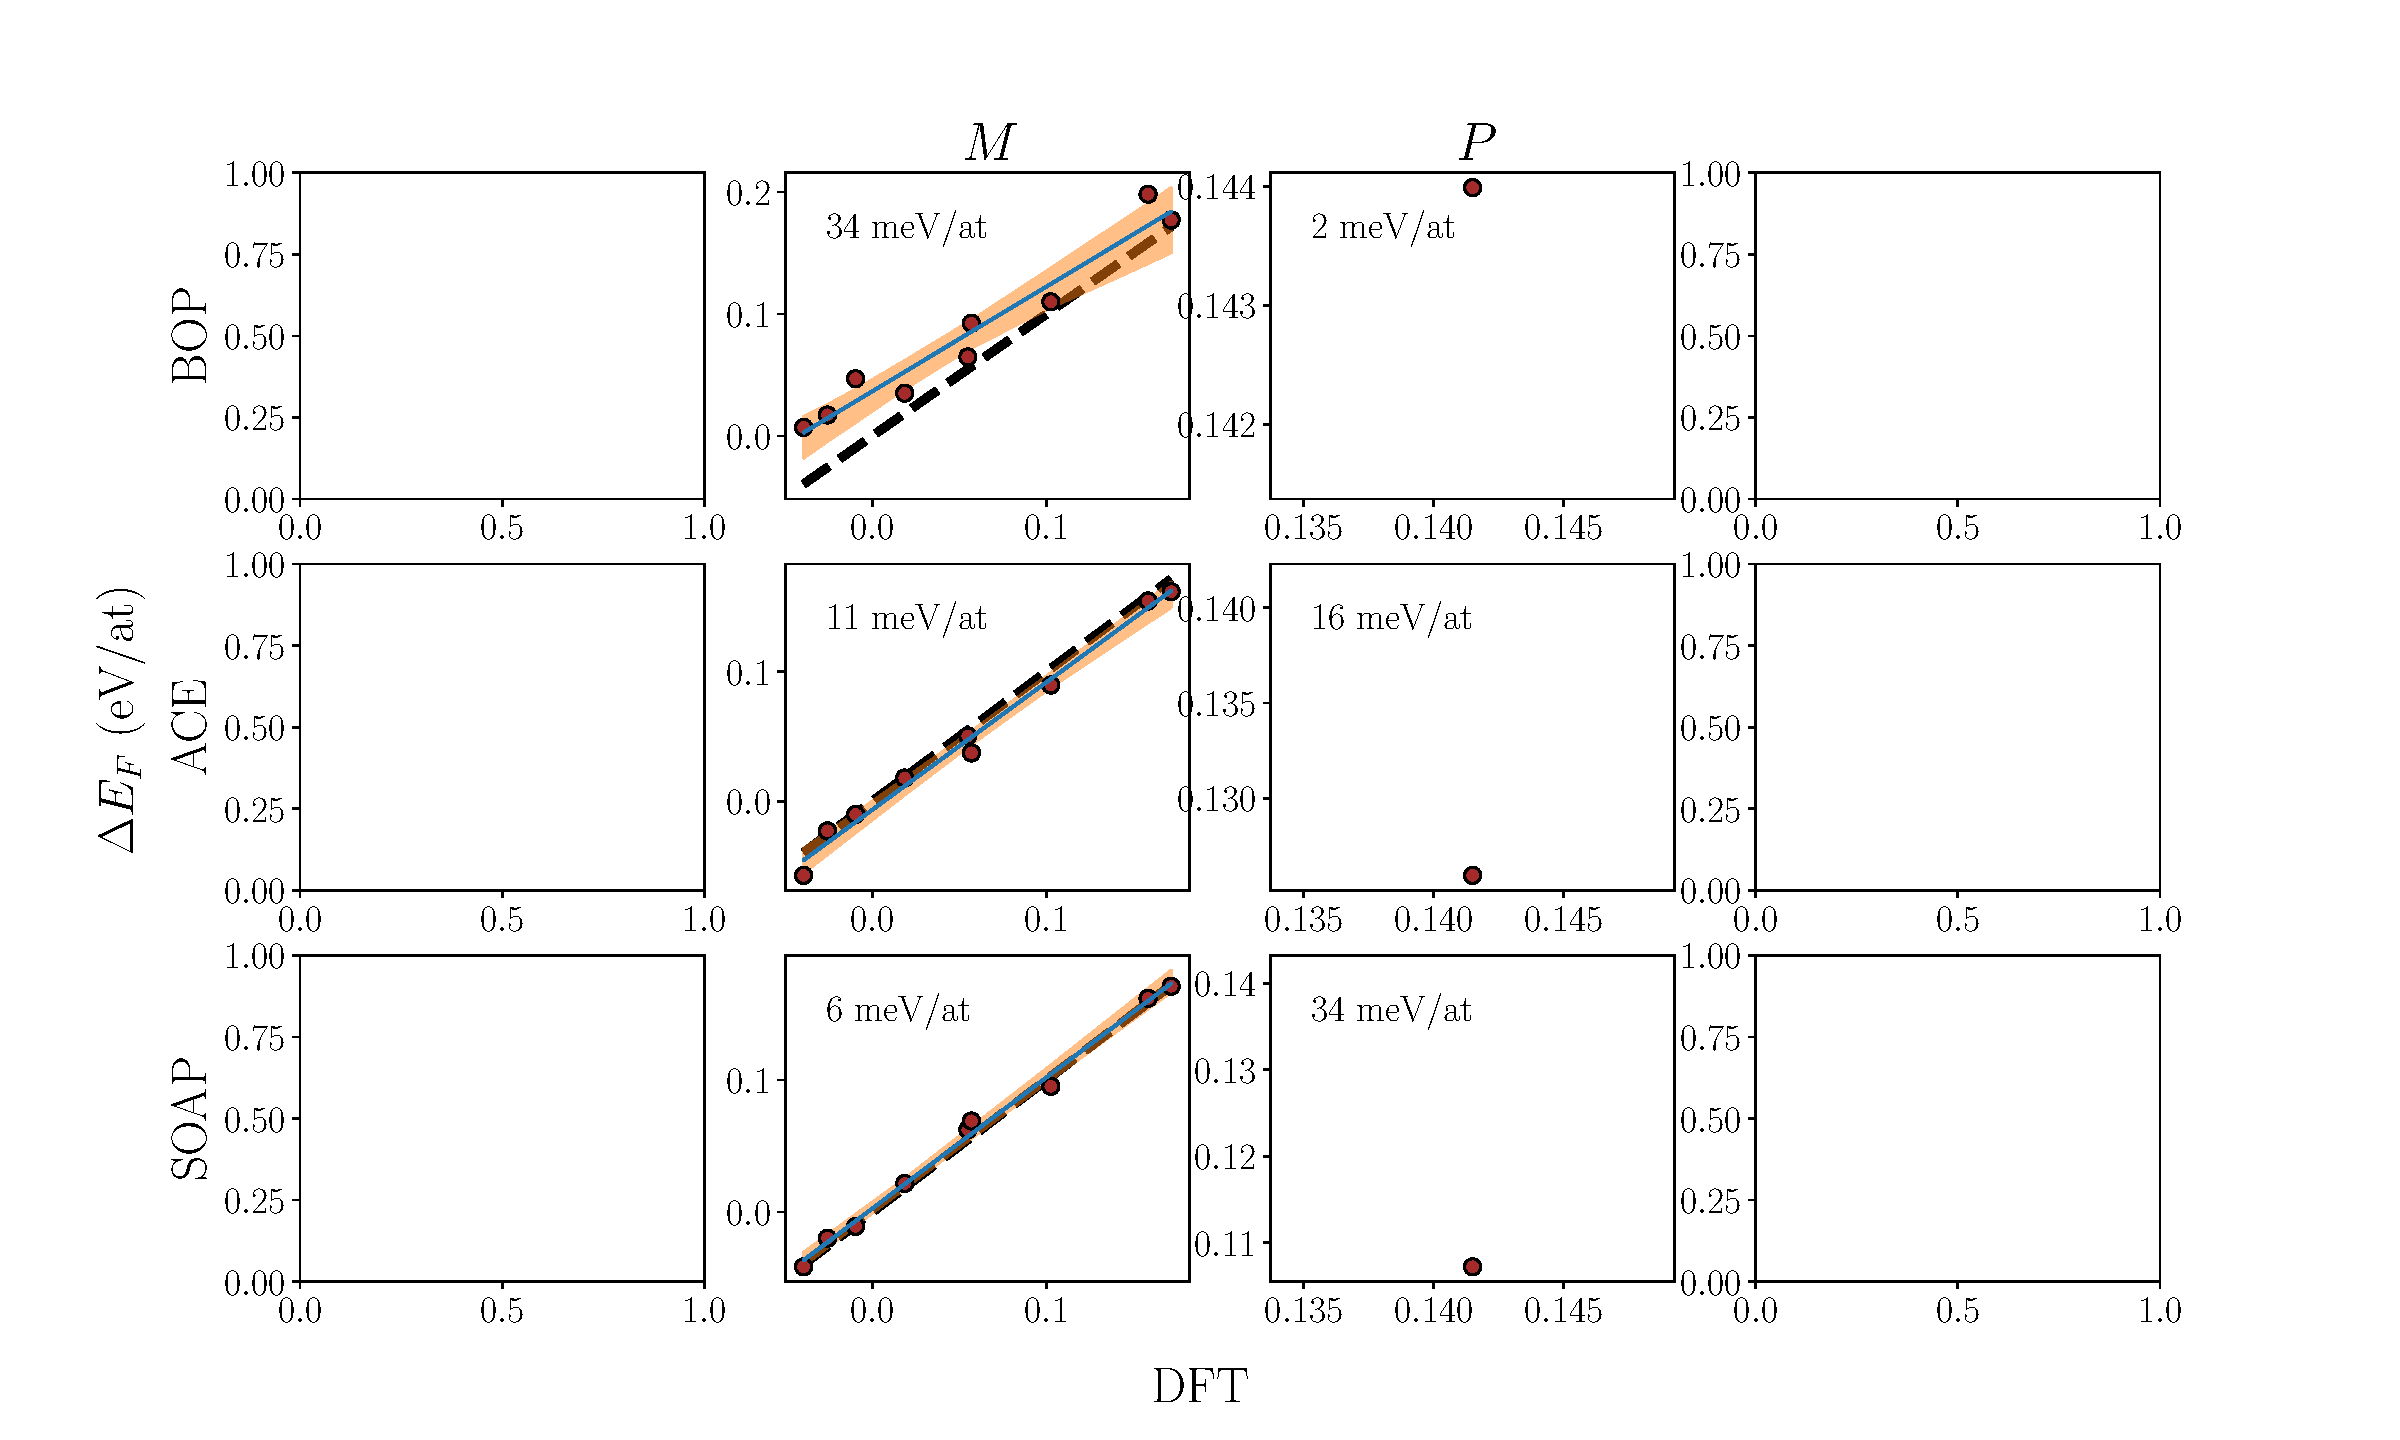
\includegraphics[width=\columnwidth]{Figure_Fe-Mo_Predictions_Validation.pdf}
\caption{Parity plots for the 70-structure external validation set, resolved by descriptor family and phase. The set contains R (19), M (11), P (12), and $\delta$ (28) structures, and the phase-resolved RMSE values span 6.0--58.4~meV/atom.}
\label{fig:validation}
\end{figure}

\begin{table}[t]
\caption{Phase-resolved external-validation RMSE values in meV/atom for the 70 held-out complex structures.}
\label{tab:validation}
\begin{tabular}{lcccc}
\toprule
Descriptor & R & M & P & $\delta$ \\
\midrule
BOP & 23.2 & 35.2 & 32.2 & 54.3 \\
ACE & 35.8 & 8.6 & 16.7 & 40.3 \\
SOAP & 12.5 & 6.0 & 16.4 & 58.4 \\
\bottomrule
\end{tabular}
\end{table}

\subsection{Thermodynamic propagation and site occupancies}

The thermodynamic results are shown in Fig.~\ref{fig:thermo} and the occupancy comparison is shown in Fig.~\ref{fig:occupancy}. Figure~\ref{fig:thermo} reports the 1700~K Gibbs free-energy curves and convex-hull construction for the R, P, M, and $\delta$ phases after the machine-learning energies were embedded in the Bragg--Williams/CEF workflow. The key numerical point is that the machine-learning error scale remained smaller than the thermal scale across the full validation range, with 58.4~meV/atom $<146.5$~meV/atom. This inequality does not remove all thermodynamic uncertainty, but it supports the use of the learned energies as an input to finite-temperature free-energy modeling. Figure~\ref{fig:occupancy} then compares R-phase occupancies against the seven experimental x-ray diffraction compositions between $x_{\mathrm{Fe}}=0.27958$ and $x_{\mathrm{Fe}}=0.37978$. The experimental occupancies were determined by Joubert and Crivello (2012) at room temperature from samples quenched from high-temperature equilibration; the Bragg--Williams calculation was performed at 1700~K. This temperature mismatch means that the comparison tests whether the machine-learning energies correctly rank the sublattice ordering tendency rather than providing a strict quantitative test of the 1700~K occupation fractions — quench kinetics and residual ordering could shift individual occupancy values by a few percent. Because each composition contains 11 experimental occupancy entries, the comparison covers 77 occupancy values distributed over the D1, D2, C1, B1, B2, and A1--A6 coordination-labeled classes. The thermodynamic workflow therefore connects the structure-energy regression problem to a more demanding observable space in which phase stability and sublattice chemistry are tested simultaneously.

A second important point is methodological rather than graphical. The training set contained only 30 complex R structures and 0 $\delta$ structures, yet the free-energy and occupancy calculations required interpolation across continuous composition variables and across the full 11-sublattice R description. The ability to perform that propagation at all depended on errors remaining within a few tens of meV/atom for the complex validation structures. If the external-validation errors had remained near the 111.4--154.8~meV/atom scale of canonical BOP or one-hot baselines, the thermodynamic curves would have been comparable to or larger than $k_{\mathrm{B}}T$ and the site-occupancy comparison would have lost meaning. The thermodynamic figures therefore serve as a stringent end-to-end validation of the descriptor and CNAV choices, not merely as a separate post-processing step.

\begin{figure}[htb]
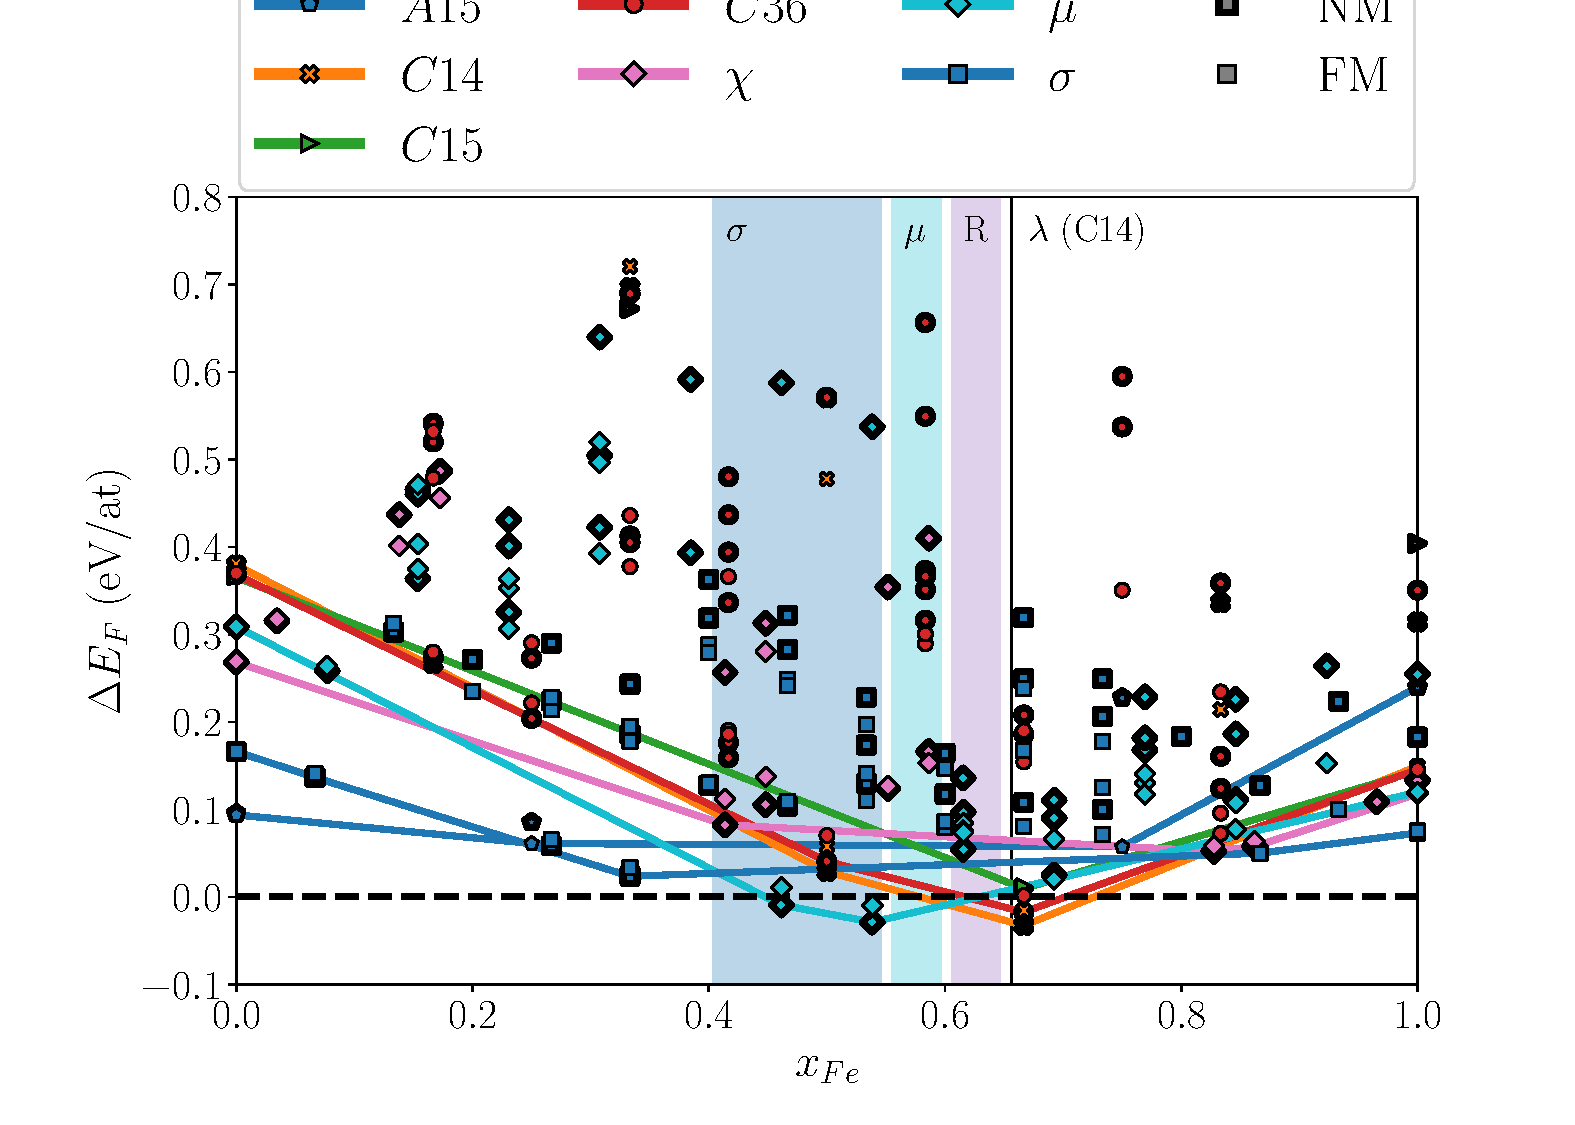
\includegraphics[width=\columnwidth]{Figure_Fe-Mo_ConvexHulls_ExpRanges_FMNM.pdf}
\caption{Gibbs free-energy curves and convex-hull construction at 1700~K for the R, P, M, and $\delta$ phases obtained from the Bragg--Williams/CEF treatment of the machine-learning energies. The thermal scale is $k_{\mathrm{B}}T=146.5$~meV/atom at 1700~K.}
\label{fig:thermo}
\end{figure}

\begin{figure}[htb]
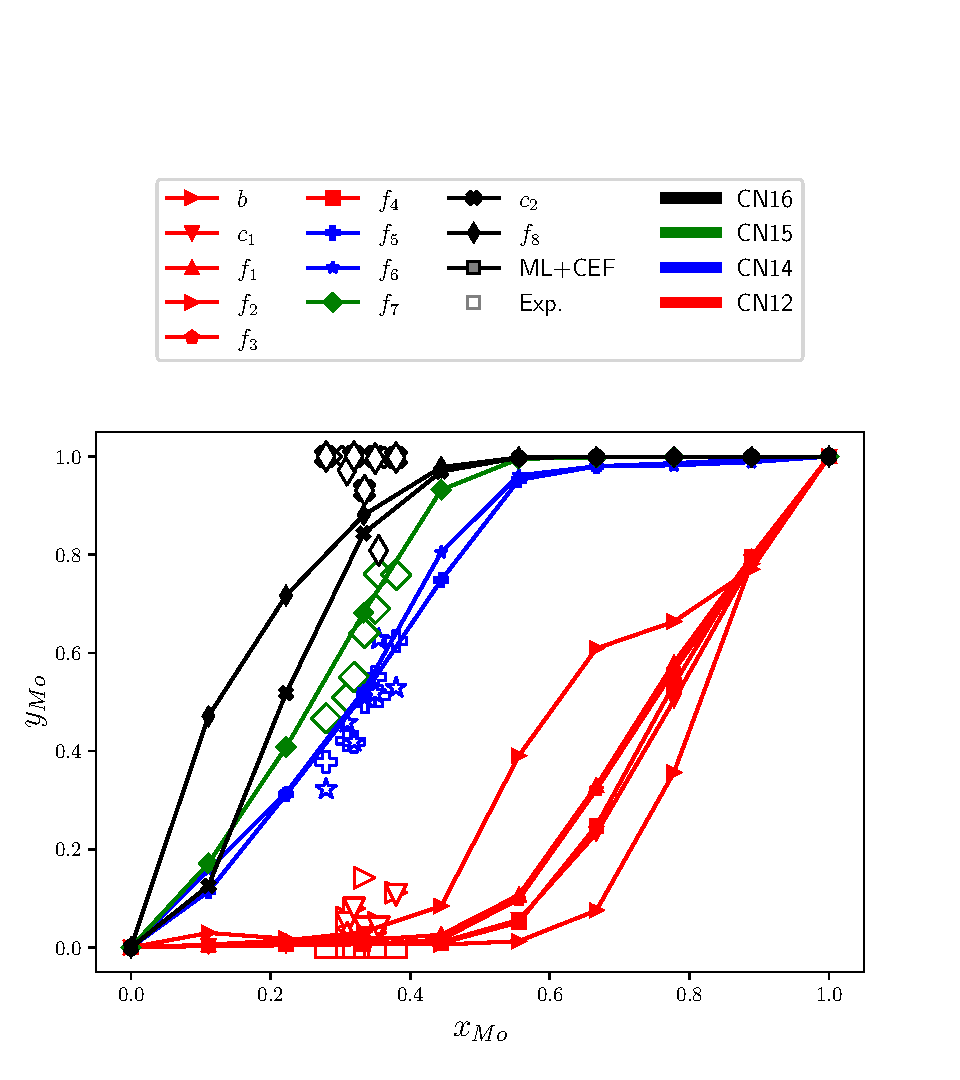
\includegraphics[width=\columnwidth]{SiteOccupancyExperimental_vs_Predictions.pdf}
\caption{Comparison between predicted R-phase site occupancies and experimental x-ray diffraction data. The figure covers seven compositions in the interval $x_{\mathrm{Fe}}=0.27958$--$0.37978$ and 11 coordination-labeled occupancy channels, giving 77 occupancy values in total.}
\label{fig:occupancy}
\end{figure}

\section{Discussion}

The combined results identify a specific transfer mechanism from simple to complex TCP phases. The best-performing BOP model is not the one with the richest global average but the one that keeps 16 site-resolved moment features, uses 0.7d projections with a 0.5 on-site contribution, and preserves coordination hierarchy through CNAV. The resulting 32\% error reduction from 34.8 to 23.5~meV/atom corresponds to an absolute gain of 11.3~meV/atom, which is 15\% of the dataset-encoding baseline of 73.9~meV/atom and therefore constitutes a physically meaningful contribution rather than a minor preprocessing gain. It indicates that the physically relevant information is carried by the coupling between local d-band descriptors and the discrete coordination classes of Frank--Kasper polyhedra. That interpretation is consistent with the canonical structure-map logic of TCP stability and with bond-order descriptions of transition-metal bonding \cite{Pettifor1995,HammerschmidtSeiser2008,Hammerschmidt2019BOPfox}. The much smaller ACE change of 1\% and intermediate SOAP change of 12\% further support the idea that CNAV is most useful when the raw descriptor does not already encode higher-order structural correlations over a broad neighborhood.

The comparison with more general machine-learning approaches highlights what is and is not claimed here. Modern interatomic-potential formalisms such as GAP, Behler--Parrinello neural networks, NequIP, MACE, and graph-based universal models have demonstrated impressive accuracy across broad materials spaces, typically with training protocols that exploit much larger local-environment databases than the 262 structure energies available here \cite{Bartok2010GAP,BehlerParrinello2007,Batzner2022NequIP,Batatia2022MACE,ChenOng2022M3GNet,Butler2018,Zuo2020}. Our result is different in emphasis: by adding chemically and crystallographically informed aggregation to DFT-quality site descriptors, we reached 19.2--23.5~meV/atom test errors and 6.0--58.4~meV/atom external-validation errors without requiring force labels, million-environment datasets, or generic graph architectures. In that sense, the present Fe--Mo study demonstrates a complementary route to data efficiency in which domain knowledge compensates for the modest dataset size of approximately 209 training structures.

The present draft also has clear limitations. The first is the energetic reference choice. The target property was referenced to non-magnetic hcp Fe and non-magnetic bcc Mo, which is fully appropriate for the repository workflow but does not remove the physical importance of magnetic effects in Fe-rich environments; the models learned from both NM and FM calculations, yet the final scalar target still inherits the non-magnetic elemental reference convention. Absolute values of predicted formation enthalpies for Fe-rich compositions would shift by approximately the difference between NM-hcp Fe and FM-bcc Fe energies ($\approx$100~meV/atom per Fe atom) if a ferromagnetic reference were adopted; the relative ordering and RMSE results are unaffected by this choice because all models are trained and evaluated on the same NM-referenced targets. The second limitation is the mean-field thermodynamic treatment. Bragg--Williams/CEF neglects short-range order and vibrational free-energy contributions beyond the adopted formulation, so agreement at 1700~K should be interpreted as evidence of useful energetic ranking rather than as a complete free-energy description \cite{Hillert2001CEF,Fries1998BWG,JoubertCrivello2012}. For TCP phases with nearest-neighbour Fe--Mo pair energies of order 10--30~meV/atom the quasi-chemical short-range-order correction is of order $w^2/(4k_{\mathrm{B}}T)\approx$~10--30~meV/atom at 1700~K, comparable to the validation RMSE of the best-performing models; both sources of uncertainty should be reduced in future work. The thermodynamic calculations were performed at 1700~K, which corresponds to the upper stability limit of the R phase in the assessed Fe--Mo binary phase diagram (stable approximately 1300--1700~K at $x_{\mathrm{Fe}}\approx 0.28$--$0.38$ according to the Joubert--Crivello CALPHAD assessment \cite{JoubertCrivello2012}); the ML calculation identifies R as the lowest Gibbs-energy phase in this composition window at 1700~K, which is consistent with the assessed diagram. The third limitation is the phase coverage. Only 30 R-phase structures were present among the 262 training structures, while the external validation included 11 M, 12 P, and 28 $\delta$ structures with 0 $\delta$ examples in training. It is therefore unsurprising that the largest validation errors appear for the most strongly extrapolative cases, namely 54.3~meV/atom for BOP and 58.4~meV/atom for SOAP on $\delta$.

These limitations immediately suggest the next steps. An active-learning extension could identify which additional DFT calculations most efficiently reduce the remaining phase-specific errors, especially in the $\delta$ manifold where 28 validation structures already expose the transfer gap \cite{Jinnouchi2019,Butler2018}. A second direction is to couple CNAV-like aggregation with force-aware models or equivariant architectures so that descriptor locality and symmetry adaptation are both retained. A third direction is thermodynamic: the present 1700~K analysis could be expanded toward a broader temperature grid and eventually to multicomponent alloy spaces once additional DFT data and CALPHAD constraints become available. The present results nevertheless establish an important baseline: the combination of site-resolved descriptor physics with coordination-aware aggregation is already sufficient to move from 232 simple TCP structures and 30 R structures to predictive modeling of 70 unseen complex configurations and to finite-temperature observables.

\section{Conclusions}

We developed a complete machine-learning workflow in which 262 TCP DFT structures, drawn from a total repository of 292 calculations, were used to train descriptor-based machine-learning models for formation enthalpies referenced to non-magnetic elemental states. Kernel ridge regression provided the best test performance, reaching 23.5~meV/atom for BOP moments with CNAV, 19.2~meV/atom for ACE, and 19.8~meV/atom for SOAP, while CNAV lowered the BOP error by 32\% from 34.8 to 23.5~meV/atom. Transfer to a separate 70-structure validation set covering R, M, P, and $\delta$ phases yielded descriptor- and phase-resolved RMSE values between 6.0 and 58.4~meV/atom, all below the 1700~K thermal scale of 146.5~meV/atom. The same learned energies were sufficiently consistent to support Bragg--Williams/CEF Gibbs free-energy calculations and comparison with 77 experimental R-phase occupancy values from seven compositions. The overall result is that chemically motivated site descriptors and crystallographically motivated CNAV aggregation provide a quantitatively effective, data-efficient route for predicting complex Fe--Mo TCP energetics and their thermodynamic consequences.

\bibliographystyle{apsrev4-2}
\bibliography{references}

\end{document}
